This chapter will delve into the applicability and efficiency of APE within the data science domain. It aims to assess whether APE can effectively generate workflows for the three selected use cases - EDA, Predictive Modeling, and Text Analysis - with a particular focus on user interactions like extension, customization, or repair of found solutions. To prevent out-of-memory errors, the use cases will be divided into multiple syntactically independent sequences. Next, the alternative ASP backend will be applied to selected tasks where potential advantages or disadvantages compared to the native APE implementation could be found. Finally, given the rising popularity of generative AI in code generation, the chapter will conclude with a brief overview of the experiments on workflow construction in the data science domain with ChatGPT \cite{ChatGPT}, Bard \cite{Bard}, and Copilot \cite{openAI2021codex}. All experiment artifacts, such as generated notebooks, their scripts, or chat histories, can be found in the repository \cite{PanRepo}.

\section{Native APE}

This section will apply the APE framework to each of the three use cases: EDA, Predictive Modeling, and Text Analysis. Additionally, APE is configured to generate up to five solutions to examine the exploration potential. The evaluation focuses not on the generated notebooks' produced content but on the user interactions with APE and the data science ontology. For this reason, the use cases' Kaggle templates are simplified by only keeping unique tool sequences that might produce technically and semantically interesting workflows - Visualizing one numeric variable will not differ in data dependencies from visualizing another numeric variable, even if the use case would usually demand it. Each of the three workflows is split into multiple constraint sets whose synthesis results are evaluated separately. This is followed by a more interpretative discussion of the discovered benefits and challenges, see \autoref{fig:native_ape_summary_bar_plot}, of applying APE in each use case.

\begin{figure}
    \centering
    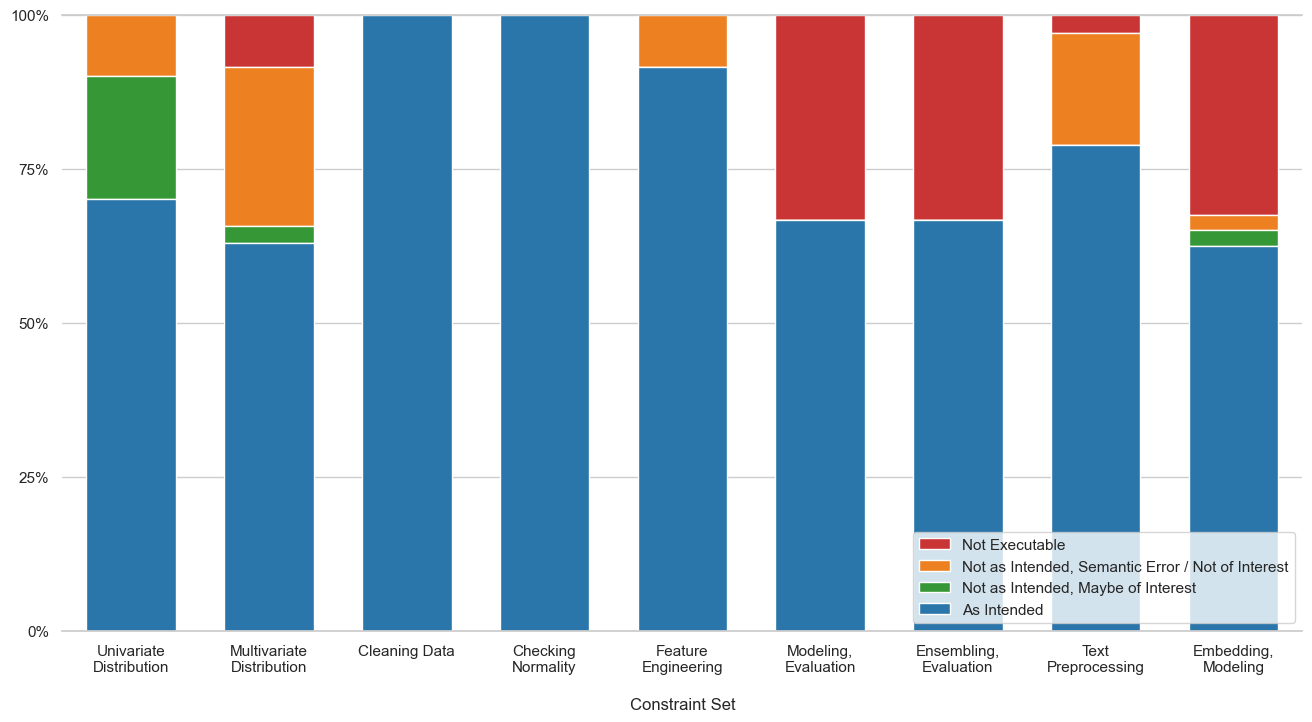
\includegraphics[width=1\linewidth]{Tex//images//native_ape_eval/constraint_set_summary.png}
    \caption{Overview of all Generated Notebook Cells across the Constraint Sets of the Three Use Cases.}
    \label{fig:native_ape_summary_bar_plot}
\end{figure}

\subsection{Exploratory Data Analysis}

Most operations in this use case draw upon the unaltered input dataset. Hence, dependencies between steps are scarce. Furthermore, in the context of EDA, there is no prioritization of specific outputs; any generated plot or statistic could be considered a valid part of the EDA artifacts, eliminating potential output data constraints or dependencies. On rare occasions where tool sequences additionally transform data, prepending or appending a descriptive tool by duplicating the chosen step will effectively capture the changes. This relative lack of inter-tool dependencies enables the workflow segmentation into the four disjunct parts introduced in \autoref{fig:usecase_housing}: 1. Exploring the Distribution of Univariate Dependent Variables, 2. Exploring Multivariate and Independent Variable Distributions, 3. Data Cleaning, and 4. Testing Statistical Assumptions.

\subsubsection{Exploring Univariate Dependent Variable Distribution}

The initial tool sequence exploring univariate distributions should compute three descriptive statistics or summaries and plot the dependent variable. Notably, no data must be passed between tools, so the constraint set is relatively simple. \autoref{table:native_ape_uni_constraints} contains the desired results and their groups of inferred APE constraints represented by their natural language templates.
\begin{table}[h]
\centering
\footnotesize
\begin{tabular}{|p{0.35\textwidth}|p{0.55\textwidth}|}
\hline
\textbf{Intention} & \textbf{Constraint} \\
\hline
Describe the input data. & Use module \texttt{describe}. \\
\hline
Plot a distribution graph of the dependent variable. & Use \texttt{Distribution} with an input of type \texttt{DependentVariable}. \\
\hline
\multirow{2}{=}{Calculate the skew and kurtosis of the dependent variable.} & Use \texttt{skew} with an input of type \texttt{DependentVariable}. \\
\cline{2-2}
& Use \texttt{kurt} with an input of type \texttt{DependentVariable}. \\
\hline
\end{tabular}
\caption{Univariate Distribution Exploration Constraints.}
\label{table:native_ape_uni_constraints}
\end{table}

The tools \verb|skew| and \verb|kurt| are defined with only two parameters: the source table and the column to calculate the statistic. Since only one table is available, supplying the type constraint for the single dependent variable column fixes the operation entirely, and hence, only one variation can be found in the solutions. Similarly, \verb|describe| also uses the table and column parameters. However, the column parameter is optional: If used, the description is limited to the specified column; if not, all numeric or non-numeric columns in the table are described. Two of the five generated workflows outline the entire data set, while the others limit themselves to a single column.

Next, the \verb|Distribution| module contains various plotting tools to visualize univariate or multivariate distributions. Furthermore, many have modes accepting parameters for additional customizations like \verb|hue| and \verb|style|. These degrees of freedom enable exploring different approaches to plotting the dependent variable distribution with APE. The results include:

\begin{figure}[h]
    \centering
    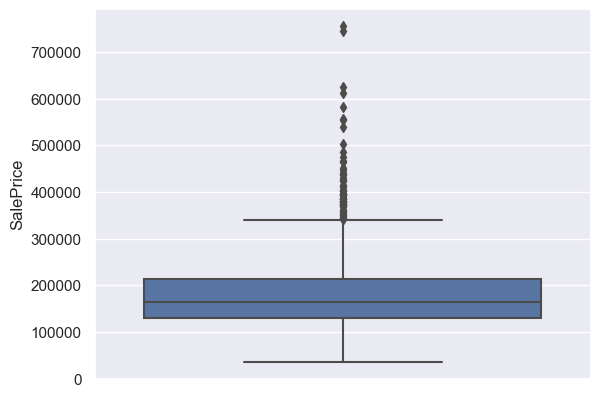
\includegraphics[width=0.5\linewidth]{Tex//images//native_ape_eval//boxplot.png}
    \caption{Generated Box Plot Showing the \texttt{SalePrice} Distribution.}
    \label{fig:native_ape_boxplot}
\end{figure}

\begin{itemize}
    \item Two box plots with the column \verb|SalePrice| across the y-axis, see \autoref{fig:native_ape_boxplot}. It is simple and gives an overview of quantiles and potential outliers. Furthermore, the plot shows the skewness in the \verb|SalePrice| column.
    \item A joint plot with the \verb|GarageArea| on the x-axis and \verb|SalePrice| on the y-axis, as shown in \autoref{fig:native_ape_jointplot_garage}. The graph shows the required distribution of the dependent variable, once via scatter and another time with a histogram. Also, the numeric independent variable \verb|GarageArea| is included, showing a seemingly linear relationship between the two columns.
    \item Another joint plot where \verb|SalePrice| is plotted against itself. The histograms on the side still show the requested \verb|SalePrice| distribution. Nonetheless, the scatter plot in the middle of the figure is arguably not adding any value.
    \item A histogram with inputs \verb|GrLivArea| and \verb|SalePrice|, as partially shown in \autoref{fig:native_ape_histogram_hue}. Here, the distribution is plotted for the ground floor living area across the different values of the dependent variable. Since \verb|SalePrice| is also numeric, the number of unique values in its column is large enough to increase the height of the legend and figure multiple times and make the supposedly discrete hues indistinguishable. While the histograms barely resemble the actual \verb|GrLivArea| distribution, they still show the increasing sale price with increasing ground floor living area values. Additionally, the figure still provides a rough idea of the distribution of the dependent variable and even shows two potential outlier bins.
\end{itemize}

\begin{figure}[h]
    \centering
    \begin{subfigure}[t]{.47\textwidth}
        \centering
        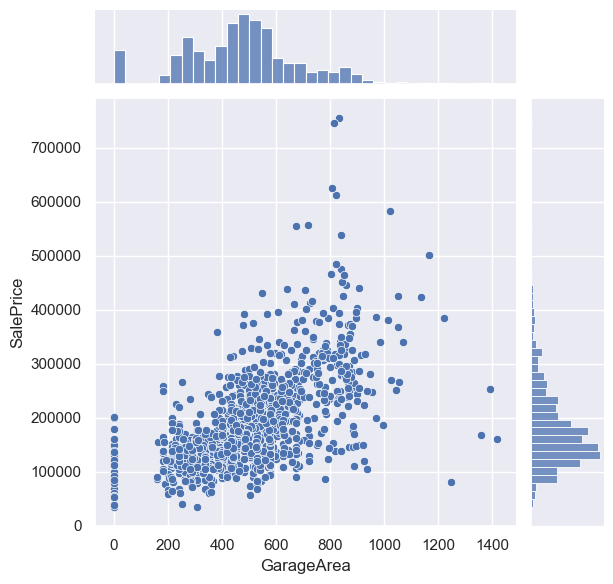
\includegraphics[width=\textwidth]{Tex//images//native_ape_eval//jointplot_garage.png}
        \caption{Joint Plot Showing the Univariate and Joint Multivariate Distributions of \texttt{SalePrice} and \texttt{GarageArea}.}
        \label{fig:native_ape_jointplot_garage}
    \end{subfigure}%
    \hfill
    \begin{subfigure}[t]{.47\textwidth}
        \centering
        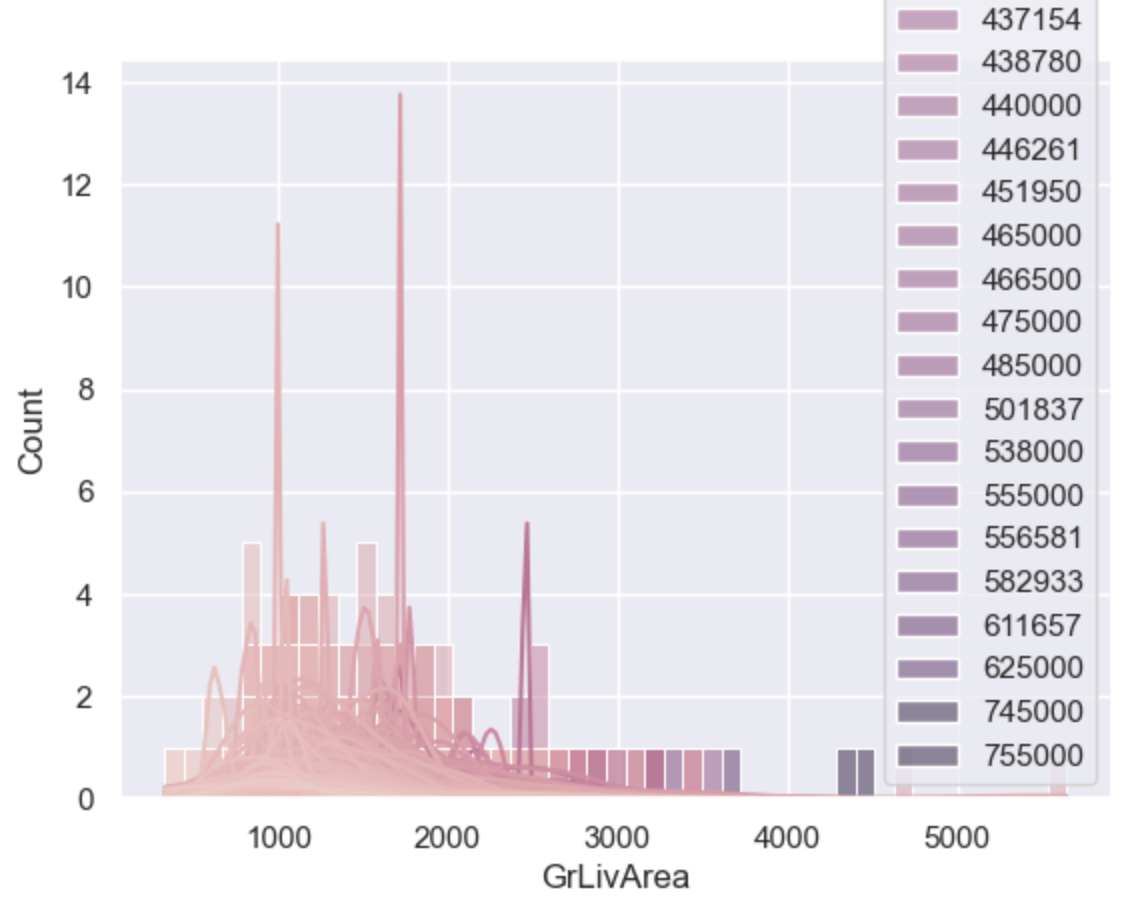
\includegraphics[width=\textwidth]{Tex//images//native_ape_eval//histogram_hue.png}
        \caption{Partial Histogram of \texttt{GrLivArea} Grouped by each Unique \texttt{SalePrice} Value with Cut-Off Legend.}
        \label{fig:native_ape_histogram_hue}
    \end{subfigure}
    \caption{Unintended EDA Results.}
    \label{fig:native_ape_double_eda_plots}
\end{figure}

\subsubsection{Exploring Multivariate and Independent Variable Distributions}\label{sec:native_ape_multi}

Including an independent variable enables the exploration aspect of APE by allowing the synthesis process to choose from various columns, thus providing semantically different outcomes. The desired results include:
\begin{itemize}
    \item Plot a relationship and a distribution graph between the dependent and an independent variable. Adjust the figure size and label rotation to the high number of axis ticks.
    \item Plot a correlation heatmap and pair plot of ten features that correlate the most with the dependent variable.
\end{itemize}
To include arbitrary integer inputs in the process, such as figure size and feature count, additional APE\_label inputs are temporarily added to the workflow configuration as outlined in \autoref{sec:native_ape_challenges}. The extensive constraint set restricting the distribution graph and heatmap tool sequences can be seen in \autoref{table:native_ape_multi_constraints}.
\begin{table}[h]
\centering
\footnotesize
\begin{tabular}{|p{0.35\textwidth}|p{0.55\textwidth}|}
\hline
\textbf{Intention} & \textbf{Constraint} \\
\hline
\multirow{2}{=}{Plot a scatter relationship graph between the dependent and an independent variable.} & Use \texttt{scatterplot} with an input of type \texttt{DependentVariable}. \\
\cline{2-2}
& Use \texttt{scatterplot} with an input of type \texttt{IndependentVariable}. \\
\hline
\multirow{8}{=}{Plot a distribution graph between the dependent and an independent variable. Also, adjust the figure size and label rotation to the high number of axis ticks.} & Use \texttt{set\_figure\_size} with an input of type \texttt{16}. \\
\cline{2-2}
& Use \texttt{set\_figure\_size} with an input of type \texttt{9}. \\
\cline{2-2}
& \texttt{set\_figure\_size} should generate an output used by \texttt{Distribution}. \\
\cline{2-2}
& Use \texttt{Distribution} with an input of type \texttt{DependentVariable}. \\
\cline{2-2}
& Use \texttt{Distribution} with an input of type \texttt{(StrColumn, IndependentVariable)}. \\
\cline{2-2}
& \texttt{Distribution} should generate an output used by \texttt{rotate\_x\_labels}. \\
\hline
\multirow{3}{=}{Plot a correlation heatmap of ten features that correlate the most with the dependent variable.} & Use \texttt{k\_most\_corr\_indep\_var\_corr\_matrix} with an input of type \texttt{DependentVariable}. \\
\cline{2-2}
& Use \texttt{k\_most\_corr\_indep\_var\_corr\_matrix} with an input of type \texttt{10}. \\
\cline{2-2}
& \texttt{k\_most\_corr\_indep\_var\_corr\_matrix} should generate an output used by \texttt{heatmap}. \\
\hline
\multirow{2}{=}{Plot a pair plot of ten features that correlate the most with the dependent variable.} & Use \texttt{pairplot} with an input of type \texttt{DependentVariable}. \\
\cline{2-2}
& Use \texttt{pairplot} with an input of type \texttt{10}. \\
\hline
\end{tabular}
\caption{Multivariate Distribution Exploration Constraints.}
\label{table:native_ape_multi_constraints}
\end{table}

Two of the five generated workflows, solutions three and five, contain faulty code and abort their executions. These errors occur during the \verb|heatmap| step, the subsequential \verb|rotate_x_labels| step that tries to use the \verb|heatmap| results, and during the \verb|pairplot| step.

The heatmap tool includes an optional pivot step, executed if the pivot columns are passed to the tool. These columns must exist in the table. However, since we removed the \verb|DataSetIndex| dimension from the type taxonomy to reduce the overall complexity, APE created workflows trying to access columns that were dropped when the \verb|k_most_corr_indep_var_corr_matrix| tool generated the correlation matrix. Even though other solutions use existing columns and, thus, generate syntactically valid workflows, the resulting notebooks do not present any relevant information: The heatmap tool is not intended to allow pivoting on correlation matrices, see \autoref{fig:native_ape_heatmap_error}. The other workflows contain the implicitly intended tool mode of the heatmap module, as shown in \autoref{fig:native_ape_heatmap_intended}.

\begin{figure}[h]
    \centering
    \begin{subfigure}[t]{.47\textwidth}
        \centering
        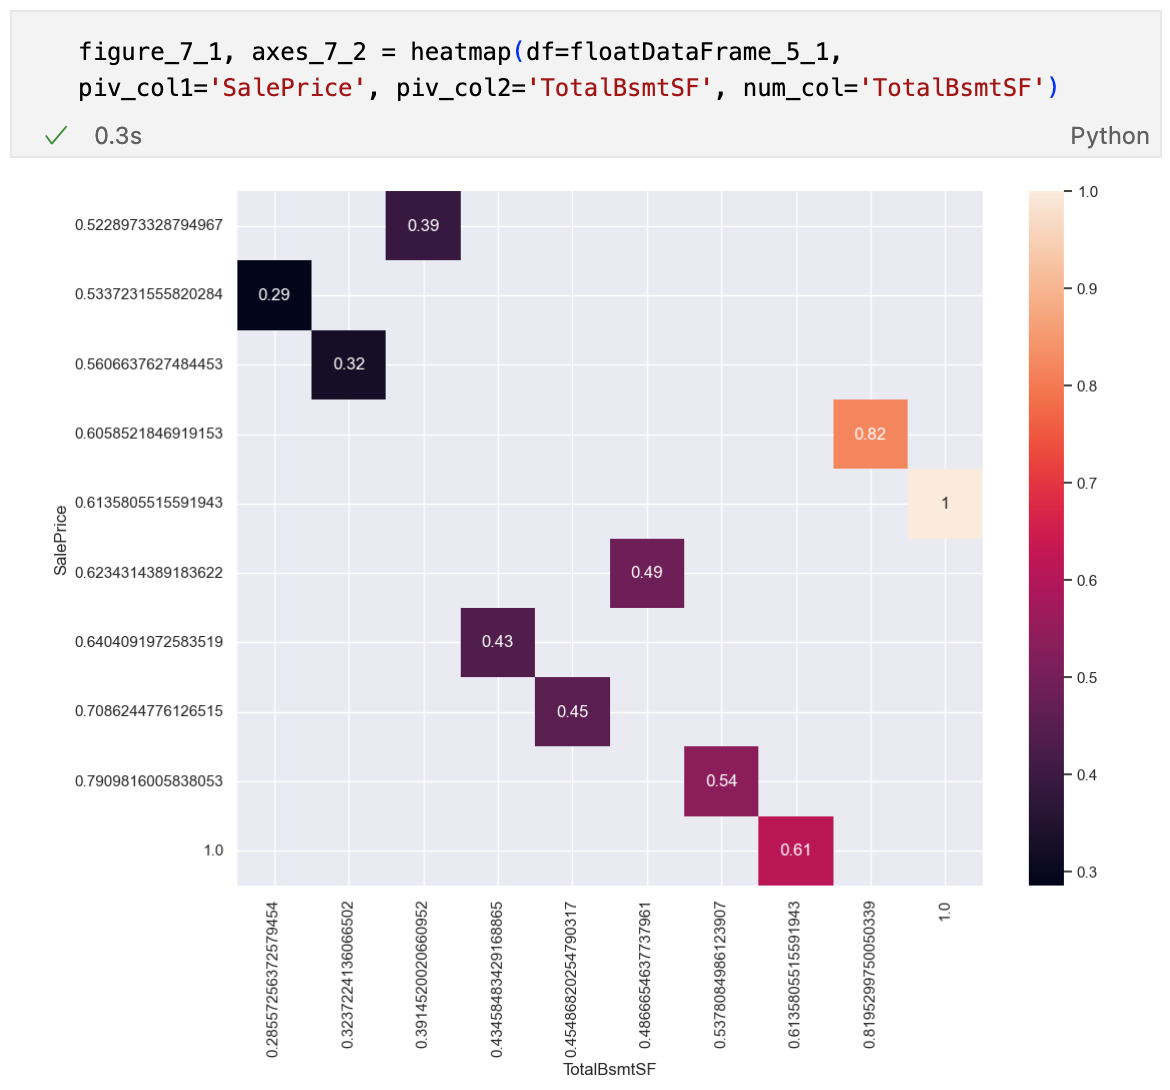
\includegraphics[width=\textwidth]{Tex//images//native_ape_eval//heatmap_error.png}
        \caption{Heatmap Generated with Pivoted Correlation Matrix.}
        \label{fig:native_ape_heatmap_error}
    \end{subfigure}%
    \hfill
    \begin{subfigure}[t]{.47\textwidth}
        \centering
        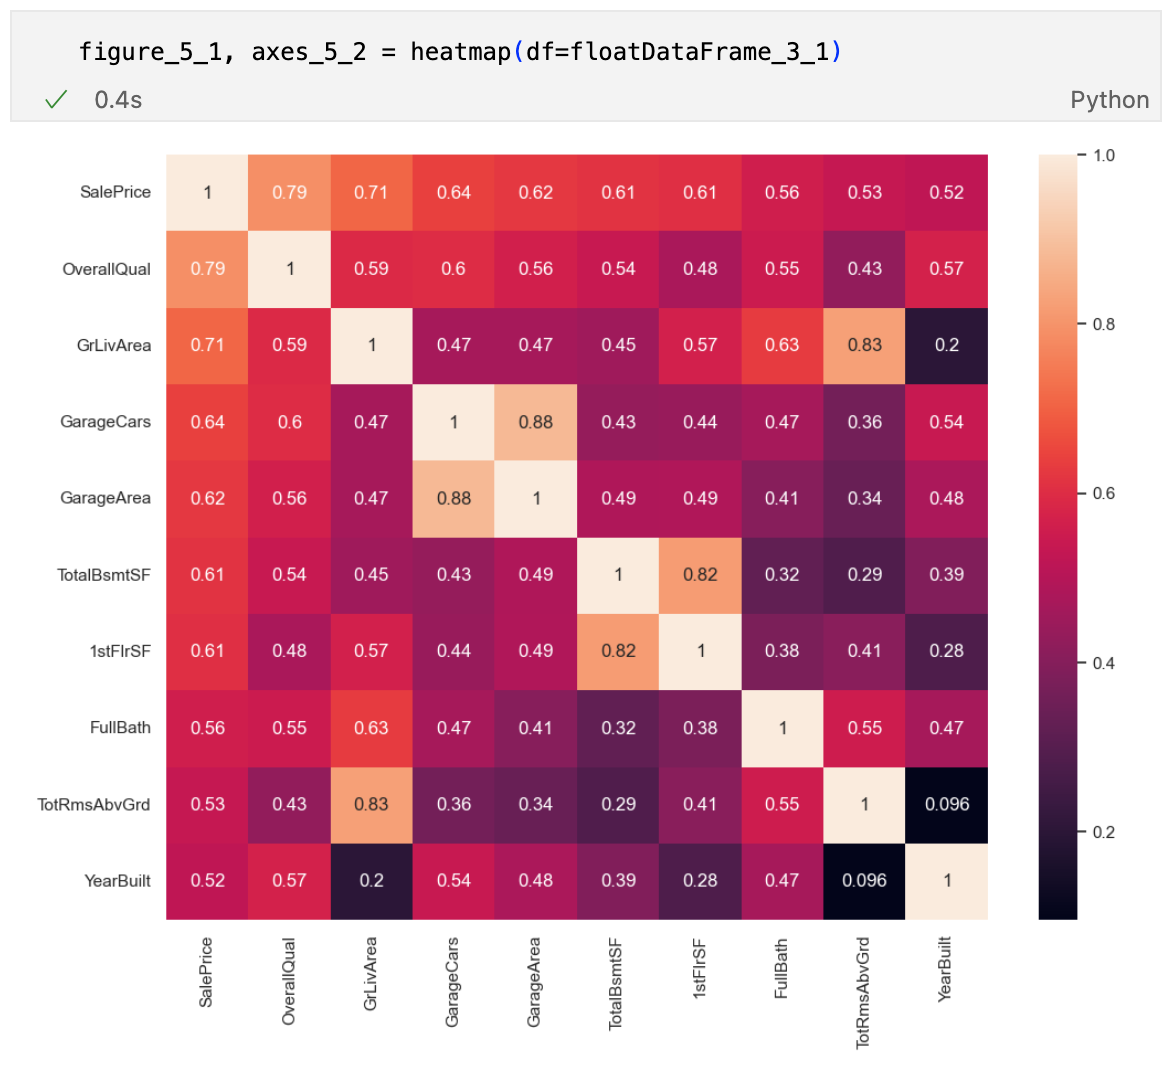
\includegraphics[width=\textwidth]{Tex//images//native_ape_eval//heatmap_intended.png}
        \caption{Intended Heatmap of Correlation Matrix.}
        \label{fig:native_ape_heatmap_intended}
    \end{subfigure}
    \caption{Heatmaps Generated by Different APE Solutions.}
    \label{fig:native_ape_double_heatmap}
\end{figure}

Next, the \verb|pairplot| module is supposed to visualize the relation of various features to each other by generating a grid of scatter plots for each column combination. Optionally, the user may provide the identifier of the dependent variable and an integer number to display only the scatter plots of the n-most correlating features. The constraints enforce at least one parameter to be assigned to the \verb|SalePrice| column. However, in one case, the column is mapped to the \verb|hue| parameter, and the notebook instead displays \(n\) features that correlate the most to the number of garages. While the scatter plots still show the requested information, the selection and order of columns seem irrelevant to the \verb|SalePrice| EDA process. The last solution aborts the tool step because the |verb|hue| is assigned to a column not available in the correlation matrix.

Another unintended result stems from the adjustment of the distribution plot. The targeted tool sequence encoded in the constraints is:
\begin{enumerate}
    \item \verb|set_figure_size| creates a new figure and axes pair.
    \item \verb|Distribution| uses the output pair and creates a resized plot.
    \item \verb|rotate_x_labels| uses the new output pair to rotate the x labels on that graph.
\end{enumerate}

The constraints imply using at least one input from \verb|set_figure_size| in Distribution. As a result, some notebooks use the generated axes, and some use the figure. In instances where there are previous plotting tools, APE may pass on one of the other outputs instead. Notably, as the last tool in the sequence, \verb|rotate_x_labels| does not receive a complete plotting pair in any of the five solutions generated.

Finally, the scatter plot tool has even more optional parameters and, hence, more unintended results in the synthesized workflows. Four notebooks contain the \verb|SalePrice| column in the y-Axis and assign various columns to the \verb|hue| parameter. The remaining notebook plots the building year against itself and colors the markers according to the sale price, as shown in \autoref{fig:native_ape_scatterplot_year}. Furthermore, it uses the correlation matrix as the source table, removing any recognizable statistical relevance from the graph. Another solution shown in \autoref{fig:native_ape_scatterplot_marker} contains the \verb|SalePrice| variable as the \verb|style| parameter, leading to Seaborn running out of distinguishable markers at a value of around 100,000.

\begin{figure}[h]
    \centering
    \begin{subfigure}[t]{.47\textwidth}
        \centering
        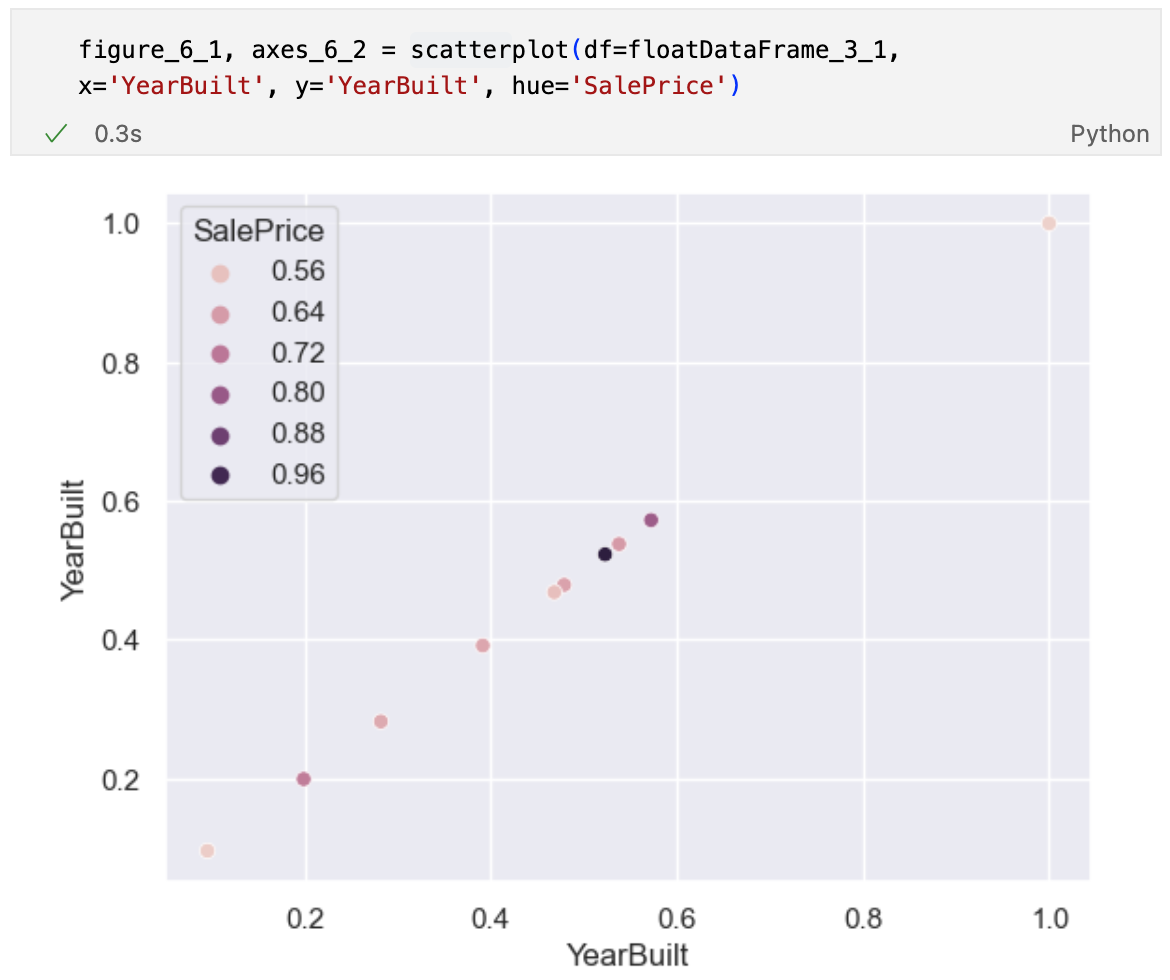
\includegraphics[width=\textwidth]{Tex//images//native_ape_eval//scatterplot_year.png}
        \caption{Scatter Plot Showing a Variable Plotted against Itself.}
        \label{fig:native_ape_scatterplot_year}
    \end{subfigure}%
    \hfill
    \begin{subfigure}[t]{.47\textwidth}
        \centering
        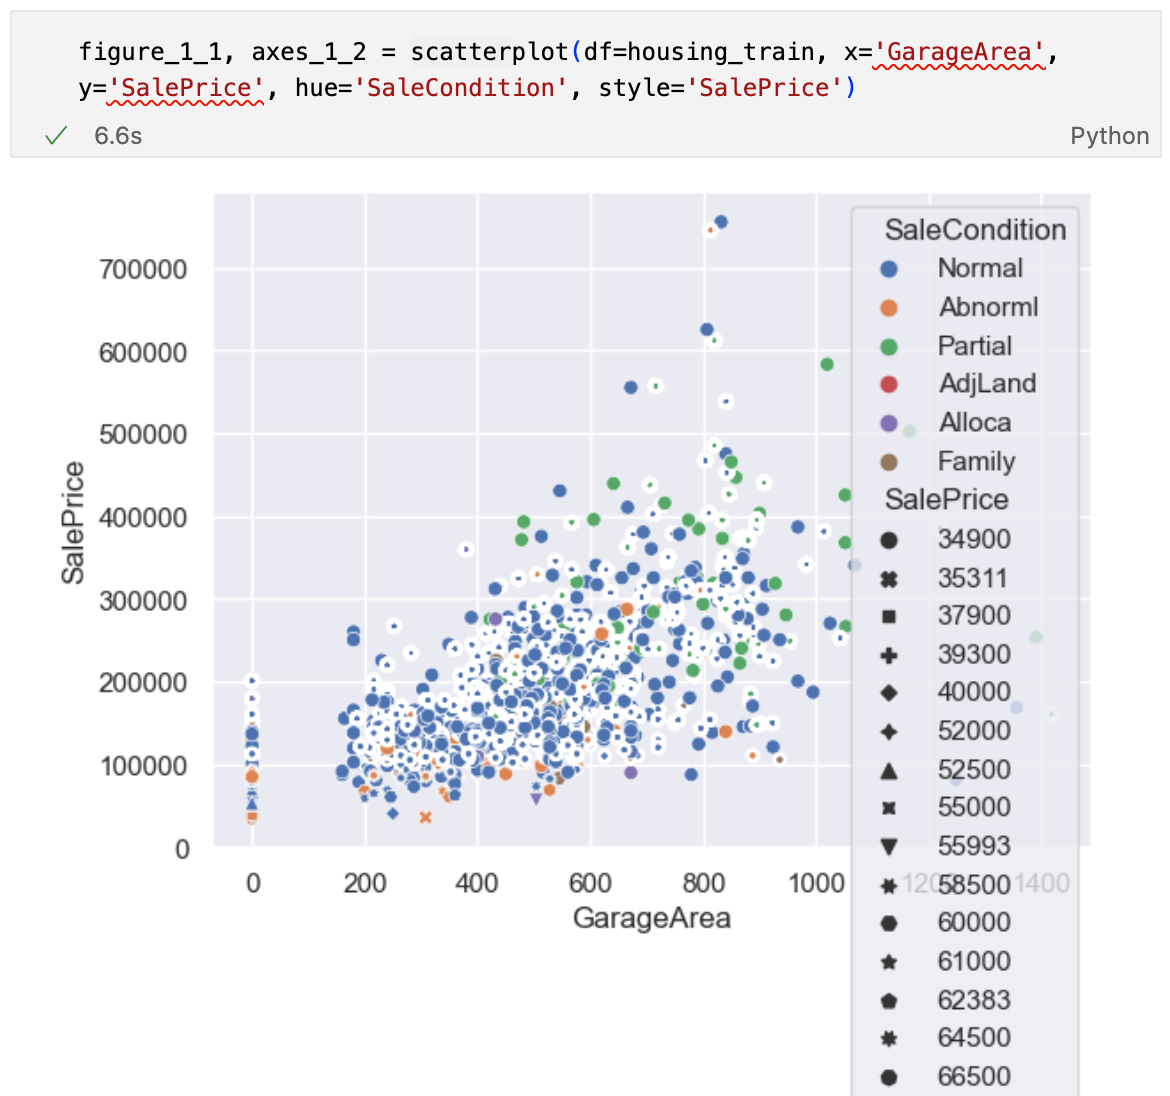
\includegraphics[width=\textwidth]{Tex//images//native_ape_eval//scatterplot_marker.png}
        \caption{Another Scatter Plot Using the \texttt{SalePrice} as the \texttt{style} Parameter.}
        \label{fig:native_ape_scatterplot_marker}
    \end{subfigure}
    \caption{Heatmaps Generated by Different APE Solutions.}
    \label{fig:native_ape_double_scatterplot}
\end{figure}

\subsubsection{Data Cleaning}

This part of the EDA use case focuses on handling missing data and outliers. As before, the tool sequence will be a simplified representation of the complete workflow that can be adapted and extended by duplicating steps and exchanging column labels. The workflow should use four tools: \verb|na_count_percentage|, \verb|drop_na_col_i|, \verb|filter_sd|, and \verb|drop_sd_i|. Usually, the user would first inspect the data and then decide to drop specific data points. However, the user can reorder these four syntactically independent tools and, thus, simplify the constraint set:
\begin{table}[h]
\centering
\footnotesize
\begin{tabular}{|p{0.35\textwidth}|p{0.55\textwidth}|}
\hline
\textbf{Intention} & \textbf{Constraint} \\
\hline
Calculate the percentage of missing data in each column. & Use module \texttt{na\_count\_percentage}. \\
\hline
Drop columns with missing data in-place. & Use module \texttt{dropna\_col\_i}. \\
\hline
Select a numeric feature and filter rows where the value might be an outlier. & Use module \texttt{filter\_sd}. \\
\hline
Drop rows with potential outliers in-place. & Use module \texttt{drop\_df\_i}. \\
\hline
\end{tabular}
\caption{Data Cleaning Constraints.}
\label{table:native_ape_data_cleaning_constraints}
\end{table}

All generated notebooks are fully executable and identical in their tool parameter mappings except for the columns selected during the outlier exploration and elimination. The in-place modifications on the input table remove the tool dependencies, such that the sequences run in any order. Nevertheless, the results differ: Removing missing values will influence the display of missing values in a subsequent step. Reordering the tool steps fixes this semantic dependency. Notably, the outlier exploration relies predominantly on experimentation with various standard deviation thresholds. However, the notebooks provide preliminary views into potential outliers without requiring user-specified values, as this parameter is already set to a default value and omitted from the tool signature.

\subsubsection{Testing Statistical Assumptions}

The last APE run of this use case represents the testing of statistical assumptions. It synthesizes workflows, checking the normality of dependent and independent variables in our dataset before and after a transformation. As most numerical transformations in our toolset have the same syntax, we will only use \verb|log| as an example in the constraints; see \autoref{table:native_ape_testing_stats_constraints}.
\begin{table}[h]
\centering
\footnotesize
\begin{tabular}{|p{0.35\textwidth}|p{0.55\textwidth}|}
\hline
\textbf{Intention} & \textbf{Constraint} \\
\hline
Apply the log transformation to some column or the entire table. & Use module \texttt{log}. \\
\hline
Check the normality of the dependent variable. & Use \texttt{normality\_plots} with an input of type \texttt{(Column, DependentVariable)}. \\
\hline
Check the normality of an independent variable. & Use \texttt{normality\_plots} with an input of type \texttt{(Column, IndependentVariable)}. \\
\hline
At least one of the normality checks should use the log-transformed data. & \texttt{log} should generate an output used by \texttt{normality\_plots}. \\
\hline
\end{tabular}
\caption{Checking Normality Constraints.}
\label{table:native_ape_testing_stats_constraints}
\end{table}

\begin{figure}[h]
    \centering
    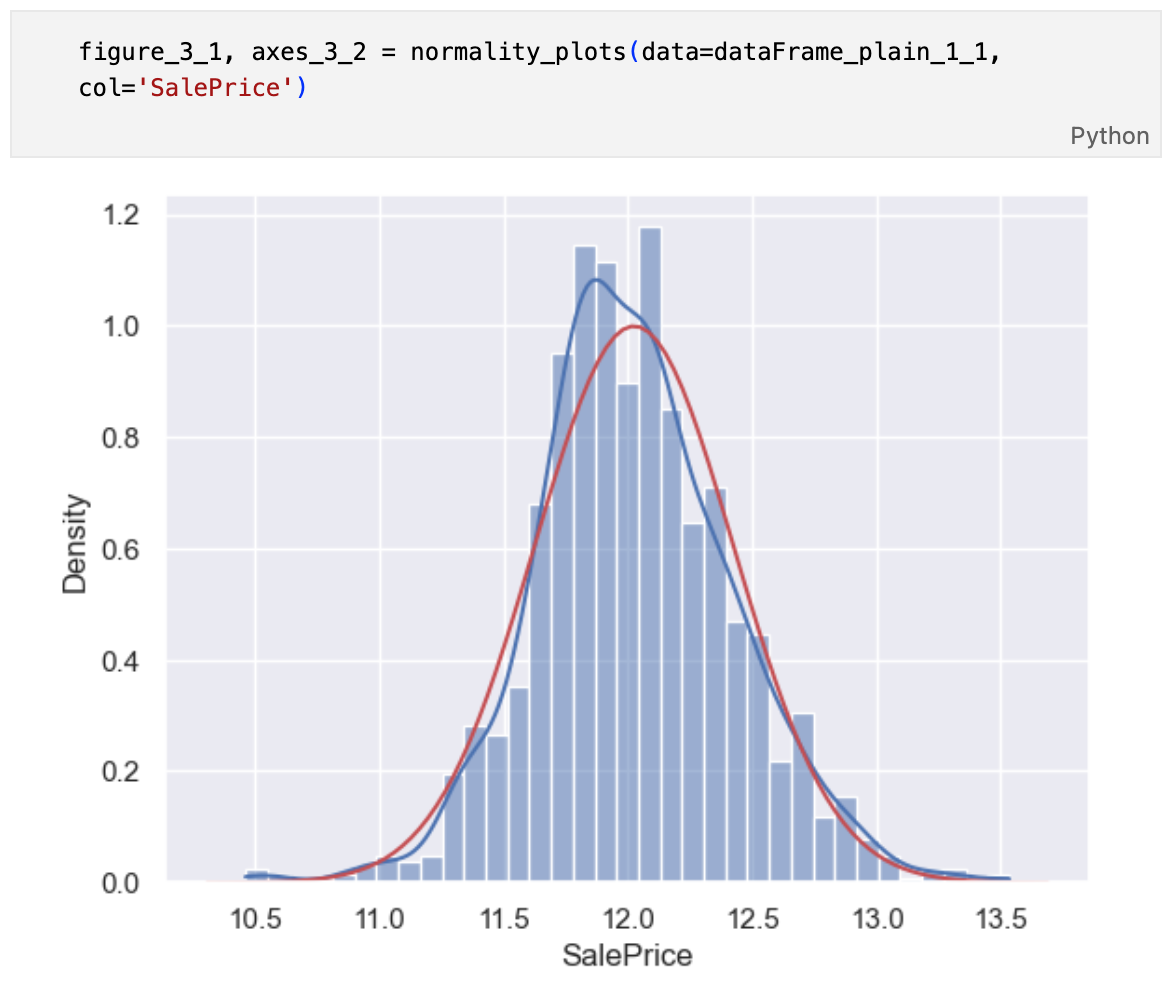
\includegraphics[width=0.5\linewidth]{Tex//images//native_ape_eval//normalityplot_log.png}
    \caption{A Normality Plot Using the Log-Transformed Data Produced in Step 1 of the Workflow.}
    \label{fig:native_ape_normalityplot}
\end{figure}

As defined by the constraints, all five solutions have a length of three, with one of the normality plots showing the selected variable after its log transformation, as shown in \autoref{fig:native_ape_normalityplot}. To examine the original and modified states for both dependent and independent variables, the constraints would have to be capable of distinguishing between multiple applications of the \verb|normality_plots function|. Adding more constraints to fix the entire tool sequence would increase the search complexity and potentially be more time-intensive than manually duplicating the required tool cells and exchanging the column parameter.

\subsubsection{Discussion}

\begin{table}[h]
\centering
\caption{Summary of Code Cells across the EDA Constraint Sets.}
\label{tab:native_ape_housing_summary}
\footnotesize
\begin{tabular}{|c|c|c|c|c|c|}
\hline
\makecell{Constraint Set} & \makecell{Steps} & \makecell{As\\Intended} & \makecell{Not as Intended,\\Maybe of Interest} & \makecell{Not as Intended,\\Semantic Error /\\Not of Interest} & \makecell{Not\\Executable} \\ \hline
\makecell{Univariate \\ Distribution} & 20 & 14 & 4 & 2 & 0 \\ \hline
\makecell{Multivariate \\ Distribution} & 35 & 22 & 1 & 9 & 3 \\ \hline
\makecell{Cleaning \\ Data} & 20 & 20 & 0 & 0 & 0 \\ \hline
\makecell{Checking \\ Normality} & 15 & 15 & 0 & 0 & 0 \\ \hline
\end{tabular}
\end{table}

Most of the synthesized notebooks are executable in their entirety, and in the few cases where errors halt the run, the notebook can be manually resumed, skipping the affected cell. \autoref{tab:native_ape_housing_summary} overviews each partial workflow's result across all five generated solutions. Only the notebooks for multivariate distribution exploration, which introduces data dependencies, are not always executable. The lack of constraints to order or directly map types to parameters leads to potentially interesting tool uses and additional dimensions in requested figures when many available columns match the parameters, as was the case in the first two APE configurations. Nevertheless, often, the information produced by these tools is presented ineffectively or unsatisfactory.

In cases of column switch-ups or incorrect use of parameters, the markdown tool notes, exemplified by \autoref{fig:native_ape_tool_tip}, enable the user to make these minor corrections. However, some tools, namely plotting tools with style options, may have many input and output parameters, creating large documentation cells interrupting the code and result displays. Nevertheless, the information provided in these cells is essential for modifying the generated notebooks. It may be possible to reformat the parameters into a table to make it easier to read.

\begin{figure}[h]
    \centering
    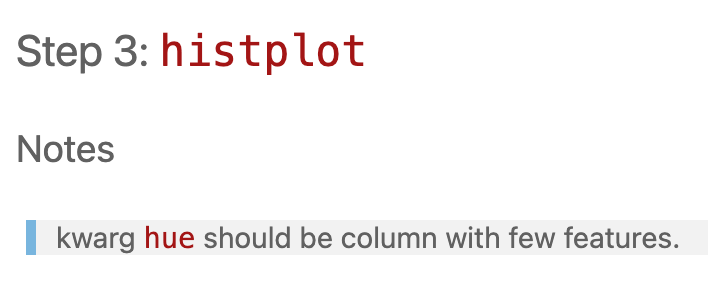
\includegraphics[width=0.5\linewidth]{Tex//images//native_ape_eval//tool_tip_hue.png}
    \caption{Tool Tip for \texttt{histplot} Hinting at Error in \autoref{fig:native_ape_histogram_hue}.}
    \label{fig:native_ape_tool_tip}
\end{figure}

If tools produce new data sets, APE often falsely assigns these tables instead of the input tables in subsequent steps. This incorrect use of different dataset types could be avoided with the \verb|DataSetIndex| dimension. Alternatively, additional constraints to explicitly control the data flow would increase the proportion of usable results. Specifically, these constraints would require the given tool to receive another's entire output.

Performing operations in-place, such as in the data cleaning solutions, increases the probability of notebooks executing successfully. This could give users the impression of a reliable workflow, even though it may disregard underlying semantic dependencies.

Most of the time, at least one notebook had the desired results for every request. Users could select these tool cells and stitch together a new notebook, fulfilling all their constraints while adding in the out-of-scope but still relevant results. Overall, the dependency and data flow sequences in this EDA use case are relatively short, resulting in any faulty steps having minimal impact on subsequent steps.

\subsection{Predictive Modeling}

The second use case trains a predictive model and thus includes a higher proportion of transformations and, hence, more dependencies than the EDA workflow. However, due to the available in-place data manipulation tools, we can split it into three partial sequences to lower the search complexity in APE and stitch the resulting notebooks back together without modifying the code cells: 1. Feature Engineering, 2. Model Training and Evaluation, 3. Ensembling and Evaluation.

\subsubsection{Feature Engineering}

This first partial workflow uses transformation and encoding tools to preprocess the titanic data set for use with sci-kit-learn's models. The constraint set for this configuration is rather extensive and detailed, as can be seen in the excerpt in \autoref{table:native_ape_feature_eng_constraints}.
\begin{table}[h]
\centering
\footnotesize
\begin{tabular}{|p{0.35\textwidth}|p{0.55\textwidth}|}
\hline
\textbf{Intention} & \textbf{Constraints} \\
\hline
\multirow{2}{=}{Extract the title prefix from the \texttt{Name} column.} & Use \texttt{extract\_i} with an input of type \texttt{Name}. \\
\cline{2-2}
& Use \texttt{extract\_i} with an input of type\linebreak\texttt{'([A-Za-z]+)\textbackslash.'}. \\
\hline
\multirow{5}{=}{Replace rare extracted titles in the \texttt{Name} column with the string \texttt{'Rare'}.} & Use \texttt{replace\_i} with an input of type \texttt{Name}. \\
\cline{2-2}
& Use \texttt{replace\_i} with an input of type \texttt{'Lady\textbar Countess\textbar Capt\textbar Col\textbar Don\textbar Dr\textbar Major\textbar Rev\textbar Sir} \linebreak \texttt{\textbar Jonkheer\textbar Dona'}. \\
\cline{2-2}
& Use \texttt{replace\_i} with an input of type \texttt{'Rare'}. \\
\cline{2-2}
& If \texttt{replace\_i} is used, \texttt{extract\_i} must have been used previously. \\
\hline
\multirow{2}{=}{Map nominal \texttt{Age} values into 20 equal-sized bins.} & Use \texttt{bin\_nominal\_i} with an input of type \texttt{Age}. \\
\cline{2-2}
& Use \texttt{bin\_nominal} with an input of type \texttt{'20'}. \\
\hline
\multirow{2}{=}{Map nominal \texttt{Fare} values into quartiles.} & Use \texttt{bin\_nominal\_q\_i} with an input of type \texttt{Fare}. \\
\cline{2-2}
& Use \texttt{bin\_nominal\_q\_i} with an input of type \texttt{'4'}. \\
\hline
Impute missing values in the column \texttt{Age} with the median. & Use \texttt{imput\_median\_i} with an input of type \texttt{Age}. \\
\hline
One-hot-encode the column \texttt{Name}. & Use \texttt{one\_hot\_encode\_i} with an input of type \texttt{Name}. \\
\hline
Encode columns only after the transformations on the underlying data are finished. & If \texttt{Encoding} is used, do not use \texttt{EDAFeatureEngineering} subsequently. \\
\hline
\end{tabular}
\caption{Feature Engineering Constraints Excerpt.}
\label{table:native_ape_feature_eng_constraints}
\end{table}

All new string and integer inputs are encoded into new APE inputs. However, the search problem with nine columns from the input data set\footnote{During the hypothetical EDA stage, the user would have decided to drop the columns \texttt{PassengerID}, \texttt{Ticket}, and \texttt{Cabin}.}, four new inputs, and a minimum of nine steps is too complex, leading to a memory error during the solving process. The adapted constraint set reduces the complexity for APE while requiring some manual changes in the notebooks by the user: The integer \verb|4| temporarily replaces \verb|20|, and two of the three near-identical one-hot-encoding steps are dropped.

All notebooks run without errors after reversing these changes in the synthesized workflow. As with previous tool sequences, unless fixed with constraints, the ordering varies and may disrupt semantic dependencies. For instance, string modifications and encodings have explicitly specified orders and occur in the correct order in all notebooks. By contrast, some notebooks unintentionally handle missing values before binning. Finally, the regular expression replacement tool uses two string parameters, which are indistinguishable except for the \verb|APE_label| dimension. Consequently, some notebooks contain steps where the search pattern substitutes the replacement string. This switch-up carries over into the subsequent one-hot-encoding steps and the final preprocessed table.

\subsubsection{Model Training and Evaluation}

The model training workflow is a well-defined sequence. Most degrees of freedom stem from the model selection or hyperparameter tuning, which are not part of this partial sequence. Since all tools implement non-in-place operations on data sets indistinguishable by APE, the data flow will be defined mainly through tool-connection constraints.
\begin{table}[h]
\centering
\footnotesize
\begin{tabular}{|p{0.35\textwidth}|p{0.55\textwidth}|}
\hline
\textbf{Intention} & \textbf{Constraints} \\
\hline
Split the input table into training and test feature and label sets. & \texttt{column\_split} should generate an output used by \texttt{train\_test\_split}. \\
\hline
\multirow{2}{=}{Train a classifier on the new training set.} & \texttt{train\_test\_split} should generate an output used by \texttt{fit\_estimator}. \\
\cline{2-2}
& Use \texttt{fit\_estimator} with an input of type \texttt{Classifier}. \\
\hline
Predict the labels of the test set. & \texttt{train\_test\_split} should generate an output used by \texttt{predict}. \\
\hline
\multirow{2}{=}{Generate a classification report for the test prediction.} & Use \texttt{classification\_report} with an input of type \texttt{Prediction}. \\
\cline{2-2}
& \texttt{train\_test\_split} should generate an output used by \texttt{classification\_report}. \\
\hline
\end{tabular}
\caption{Modeling and Evaluation Constraints.}
\label{table:native_ape_modeling_constraints}
\end{table}

None of the resulting notebooks are free of errors. While the first three steps of every workflow, initialization of a classifier, shown in \autoref{fig:native_ape_init_classifier}, and the train-test-split sequence run as intended, none of the fitting and evaluation calls are executable. Like the graph customization tools, these require multiple types to be passed between them:
\begin{itemize}
    \item \verb|train_test_split| generates four outputs: a training feature table, a test feature table, a training label series, and a test label series.
    \item \verb|fit_estimator| requires a table and series of equal length. However, without the dimension, \verb|DataSetIndex| training and test sets are indistinguishable by APE, leading to potentially inconsistent numbers of samples. Furthermore, the tool-connection constraint only requires the \verb|fit_estimator| tool to use one of the \verb|train_test_split| outputs. If, as exemplified by \autoref{fig:native_ape_fit_estimator_error}, the data set split produced the training table, the label series might be from a previous tool.
    \item \verb|predict| only uses one data set input and runs in all notebooks after fixing the other cells.
    \item \verb|classification_report| has the same data set parameter types as the tool \verb|fit_estimator|; thus, their cells have similar error sources.
\end{itemize}
\begin{figure}
    \centering
    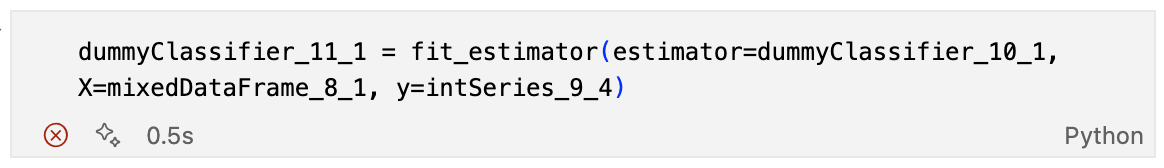
\includegraphics[width=0.5\linewidth]{Tex//images//native_ape_eval//fit_estimator.png}
    \caption{Faulty Notebook Cell Fitting the Estimator with an Incompatible Matrix-Vector Pair.}
    \label{fig:native_ape_fit_estimator_error}
\end{figure}

\subsubsection{Ensembling and Comparison}

Ensembling enables the user to request an arbitrary number of models for aggregation. To address this obstacle related to explicit parameters in tool modes, as discussed in \autoref{sec:input_labels}, the factory tool for basic ensemble models employs a single string list of model identifiers and combines their constructor calls as shown in \autoref{fig:native_ape_init_voting_classifier}. The user can alter the ensembled models by adjusting this string list following the tooltips provided. The APE configuration for training an ensemble model and comparing it to the baseline resembles that of basic models, with the sole addition including a string model list as an input. As a result, all five generated notebooks contain similar faulty \verb|split-train-predict-evaluate| tool sequences.

\subsubsection{Discussion}
\begin{table}[h]
\centering
\caption{Summary of Code Cells across the Predictive Modeling Constraint Sets.}
\label{tab:native_ape_titanic_summary}
\footnotesize
\begin{tabular}{|c|c|c|c|c|c|}
\hline
\makecell{Constraint Set} & \makecell{Steps} & \makecell{As\\Intended} & \makecell{Not as Intended,\\Maybe of Interest} & \makecell{Not as Intended,\\Semantic Error /\\Not of Interest} & \makecell{Not\\Executable} \\ \hline
\makecell{Feature\\Engineering} & 35 & 32 & 0 & 3 & 0 \\ \hline
\makecell{Modeling,\\Evaluation} & 30 & 20 & 0 & 0 & 10 \\ \hline
\makecell{Ensembling,\\Evaluation} & 30 & 20 & 0 & 0 & 10 \\ \hline
\end{tabular}
\end{table}

Variable user-defined inputs work well with the \verb|APE_labels|, as shown by the feature engineering configuration change in the first sequence and the classifier initialization steps in the last two, which use predefined strings with no source tool or user input strings. Notably, the implicit dimension encodes potentially arbitrary parameter values outside the data science ontology while still being documented by the markdown cells; see \autoref{fig:native_ape_double_init_clf}.

\begin{figure}[h]
    \centering
    \begin{subfigure}[t]{.47\textwidth}
        \centering
        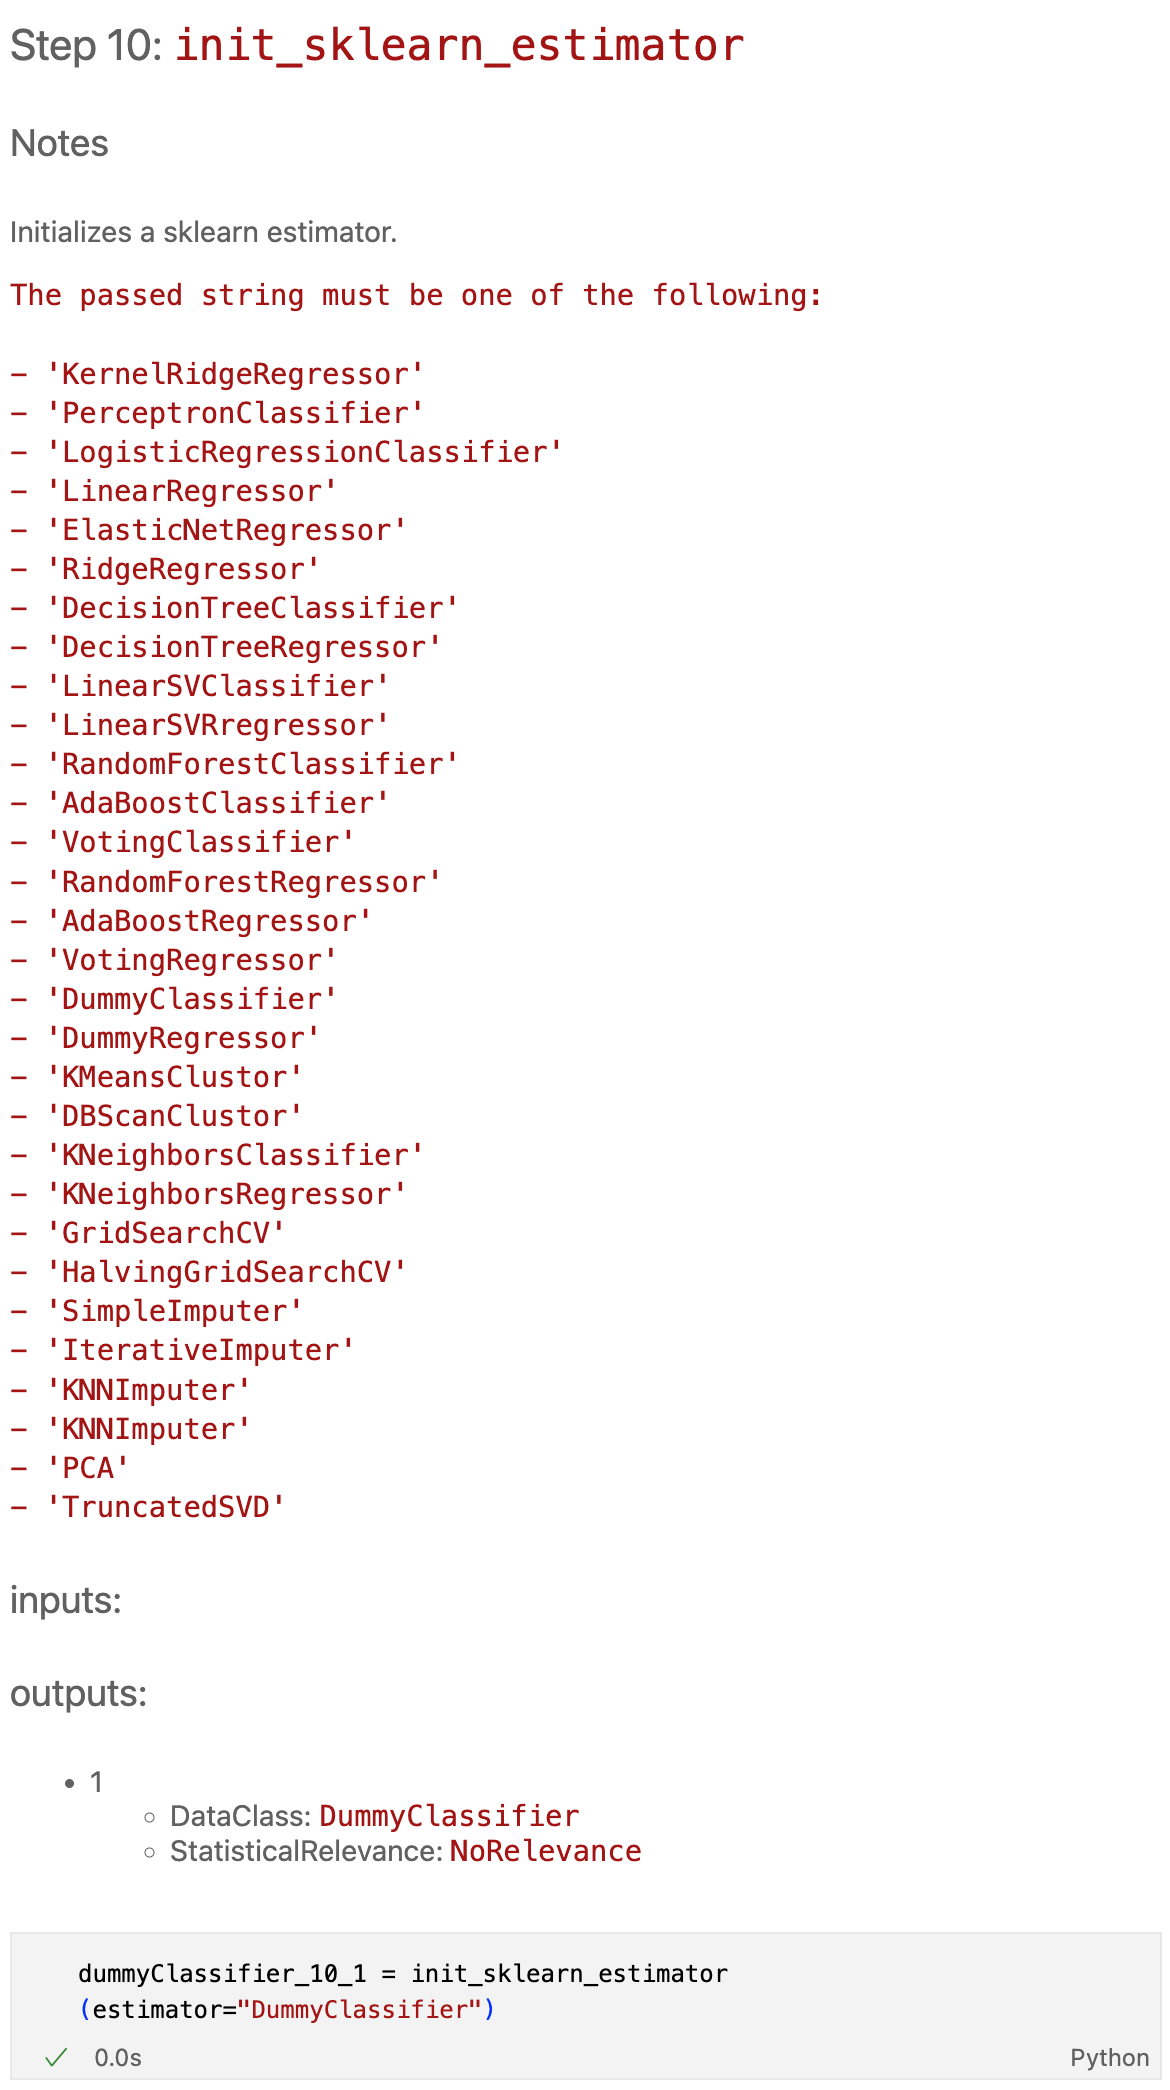
\includegraphics[width=\textwidth]{Tex//images//native_ape_eval//init_classifier.png}
        \caption{Initialization of a Model with User-Defined String Inputs.}
        \label{fig:native_ape_init_classifier}
    \end{subfigure}%
    \hfill
    \begin{subfigure}[t]{.47\textwidth}
        \centering
        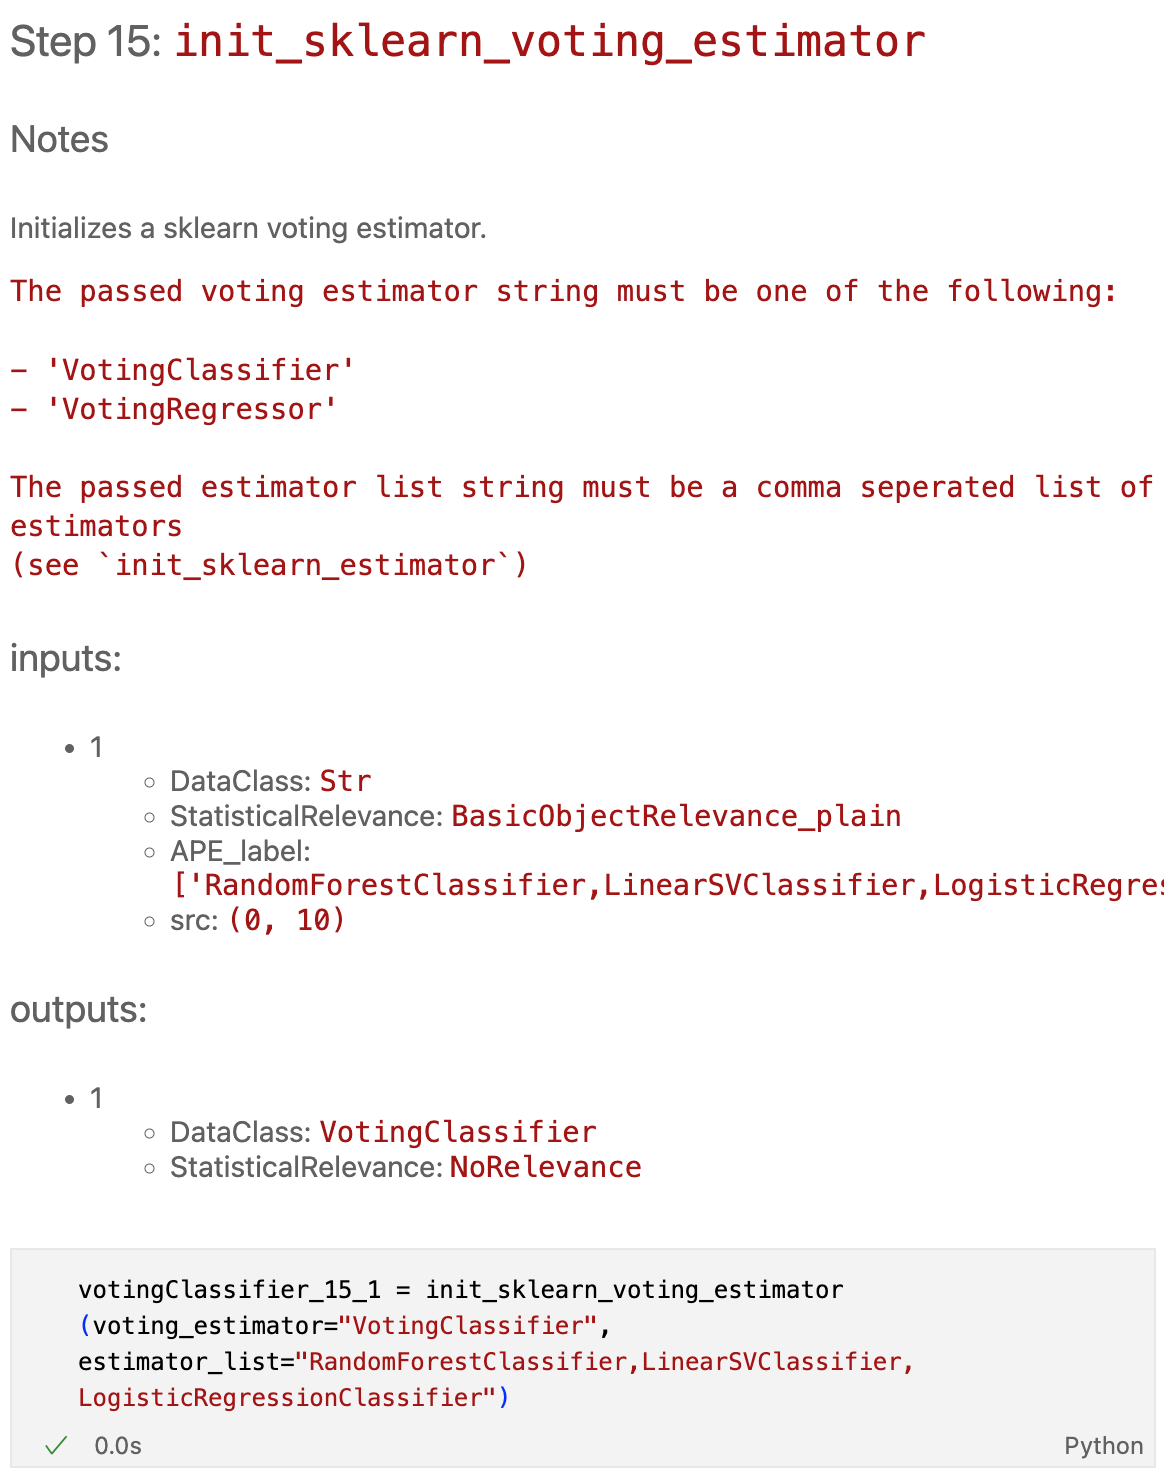
\includegraphics[width=\textwidth]{Tex//images//native_ape_eval//init_voting_classifier.png}
        \caption{Passing of a Model List Parameter as a String Input.}
        \label{fig:native_ape_init_voting_classifier}
    \end{subfigure}
    \caption{Model Initialization Code Cells with Detailed Markdown Annotations.}
    \label{fig:native_ape_double_init_clf}
\end{figure}

The rigid data flow structure in modeling workflows necessitates the user to compose a more detailed set of constraints than earlier APE configurations. Despite this effort, the received notebooks may contain invalid modeling solutions; see \autoref{tab:native_ape_titanic_summary}. Specifically, the feature engineering tool sequences use in-place transformations and, hence, are less vulnerable to unexpected parameter assignments. In contrast, training and evaluating a model generates separate data sets that might not be distinguishable with taxonomy terms. The extensive and technical nature of the applied constraints, even with the abstraction layer provided by the ontology, could make manual notebook coding a more practical and effective approach. Moreover, while varying sub-tools and column mappings proved beneficial in other tool sequences, such flexibility would undermine the statistical significance of the \verb|split-train-predict-evaluate| sequence if parameters were swapped indiscriminately.

\subsection{Text Analysis}

Lastly, the IMBD text-based dataset is a test for assessing APEs and the data science ontology's proficiency in generating workflows that process complex data types opaque to the user and more challenging to interpret within the notebook than earlier data frame types. Following the Kaggle template, the unstructured review data undergoes preprocessing before model training. The workflow is split into two segments: 1. Text Preprocessing and 2. Embedding and Modeling.

\subsubsection{Text Preprocessing}

The generated tool sequence will modify the data for the later embedding and modeling steps. Since these workflows are developed separately, all input transformations must operate in-place to preserve the other workflows' data independence, similar to the feature engineering section of the previous use case. Additionally, the data set only has one feature column: the review texts. Thus, constraints ordering the steps must be supplied to comply with the tools' dependencies while modifying this variable.

\begin{table}[h]
\centering
\footnotesize
\begin{tabular}{|p{0.35\textwidth}|p{0.55\textwidth}|}
\hline
\textbf{Intention} & \textbf{Constraints} \\
\hline
Extract text from HTML in the review column. & Use \texttt{get\_text\_from\_html\_i} with an input of type \texttt{review}. \\
\hline
\multirow{3}{=}{Next, expand abbreviations in the review text.} & If \texttt{get\_text\_from\_html\_i} is used, the next module in the sequence should be \texttt{expand\_abbr\_i}. \\
\cline{2-2}
& Use \texttt{expand\_abbr\_i} with an input of type \texttt{'abrev.json'}. \\
\cline{2-2}
& Use \texttt{expand\_abbr\_i} with an input of type \texttt{review}. \\
\hline
\multirow{4}{=}{Next, remove any non-alphabetical characters in the review text.} & If \texttt{expand\_abbr\_i} is used, the next module in the sequence should be \texttt{replace\_re\_i}. \\
\cline{2-2}
& Use \texttt{replace\_re\_i} with an input of type \texttt{review}. \\
\cline{2-2}
& Use \texttt{replace\_re\_i} with an input of type \texttt{'[\textasciicircum a-zA-Z]'}. \\
\cline{2-2}
& Use \texttt{replace\_re\_i} with an input of type \texttt{' '}. \\
\hline
\multirow{2}{=}{Next, lemmatize the review text.} & If \texttt{replace\_re\_i} is used, the next module in the sequence should be \texttt{lemmatize\_i}. \\
\cline{2-2}
& Use \texttt{lemmatize\_i} with an input of type \texttt{review}. \\
\hline
\multirow{2}{=}{Plot a word cloud from the review text as the last step.} & Use \texttt{plot\_wordcloud} as the last module in the solution. \\
\cline{2-2}
& Use \texttt{plot\_wordcloud} with an input of type \texttt{review}. \\
\hline
\end{tabular}
\caption{Text Preprocessing Constraints Excerpt.}
\label{table:native_ape_text_processing_constraints}
\end{table}

Among the five produced solutions, only two have a length of six steps, the minimum for this constraint set. The subsequent three workflows incorporate an additional seemingly arbitrarily chosen tool, leading to one notebook with incorrect parameter mappings. Another prepends the \verb|train_test_split| tool and occasionally references the wrong table for its operations. The final workflow among the longer ones also includes the \verb|train_test_split| module but disregards the output in the following tool cells. Conversely, the two minimal notebooks are identical except for the arrangement of parameters in the one tool using two string parameters that APE cannot differentiate with the data science ontology: \verb|replace_re_i|. The interchanged replacement patterns substitute whitespace characters with the intended search pattern. Nevertheless, the result remains interpretable, as seen in the comparison in \autoref{fig:native_ape_double_wordcloud}, and correcting this manually is relatively straightforward. Either way, the time consumed by APE's runtime or by manual adjustments to the notebooks pales in comparison to the duration required to process the text in 50,000 reviews\footnote{The spelling correction step is exceptionally time intensive and runs for multiple hours on the Apple M1 Max chip.}.

\begin{figure}[h]
    \centering
    \begin{subfigure}[t]{.47\textwidth}
        \centering
        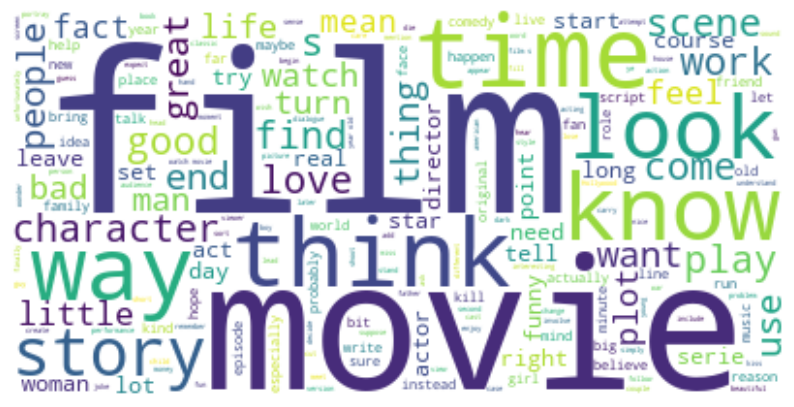
\includegraphics[width=\textwidth]{Tex//images//native_ape_eval//wordcloud_intended.png}
        \caption{The Intended Review Text Word Cloud.}
        \label{fig:native_ape_wordcloud_intended}
    \end{subfigure}%
    \hfill
    \begin{subfigure}[t]{.47\textwidth}
        \centering
        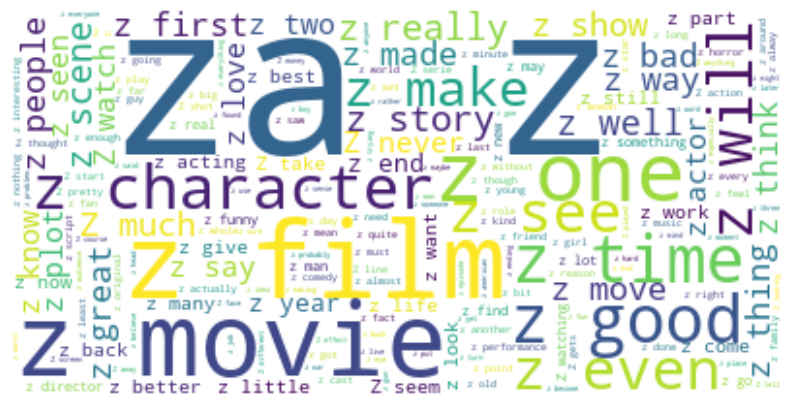
\includegraphics[width=\textwidth]{Tex//images//native_ape_eval//wordcloud_swap.png}
        \caption{The Word Cloud Generated with Swapped Substitution Patterns.}
        \label{fig:native_ape_wordcloud_swap}
    \end{subfigure}
    \caption{Wordclouds Generated by Different Solutions.}
    \label{fig:native_ape_double_wordcloud}
\end{figure}

\subsubsection{Embedding and Modeling}

The modeling workflow for textual data is similar to the basic one in that it requires the \verb|split-train-predict-evaluate| sequence. However, it further necessitates embedding the textual column into numeric matrices before the model can be trained. This embedding is fitted and applied to the training data and then reapplied to the test data for evaluation. These novel data flow requirements are added to an already fragile modeling data dependency set.

\begin{table}[h]
\centering
\footnotesize
\begin{tabular}{|p{0.35\textwidth}|p{0.55\textwidth}|}
\hline
\textbf{Intention} & \textbf{Constraints} \\
\hline
\multirow{2}{=}{Embed training review text using \texttt{Word2Vec}.} & \verb|train_test_split| should generate an output used by \verb|embed_text_word2vec|. \\
\cline{2-2}
& Use \verb|embed_text_word2vec| with an input of type review. \\
\hline
\multirow{2}{=}{Embed the test review data using the trained \texttt{Word2Vec} model.} & Use \verb|embed_text_word2vec| with an input of type \verb|Word2Vec|. \\
\cline{2-2}
& \verb|embed_text_word2vec| must have used \verb|train_test_split| prior to it. \\
\hline
\multirow{2}{=}{Train a classifier using the embedded training data.} & \verb|embed_text_word2vec| should generate an output used by \verb|fit_estimator|. \\
\cline{2-2}
& Use \verb|fit_estimator| with an input of type \verb|Classifier|. \\
\hline
\multirow{2}{=}{Predict the labels of embedded test set.} & \verb|embed_text_word2vec| should generate an output used by \verb|predict|. \\
\cline{2-2}
& \verb|fit_estimator| should generate an output used by \verb|predict|. \\
\hline
\end{tabular}
\caption{Text Classification Constraints Excerpt.}
\label{table:native_ape_text_classification_constraints}
\end{table}

This APE configuration generates suboptimal solutions similar to the earlier modeling and evaluation scenario. None of the notebooks are entirely executable; four of the five proposed workflows mismatch data inputs in the model fitting step and one in the evaluation step. The only tool sequences generated reliably have their order and input parameters fixed by constraints. Additionally, repairing the faulty code cells and further extending the notebook is more convoluted than in the previous modeling workflow. In the case of basic tables, users may directly inspect the schema and content of passed parameters to identify the issues. However, interpreting the embedded text matrices presents a difficult task to the user due to their structure. These matrices are often characterized by their large size, sparsity, high dimensionality, and lack of a direct, identifiable connection to their originating texts, as exemplified in \autoref{code:native_ape_eval_embedding}.

\begin{lstlisting}[language=python, caption=Embedding Matrix of Review Texts., label=code:native_ape_eval_embedding]
array([[-0.14810246,  0.21811058, ..., -0.16859908,
         0.17599331,  0.24811591],
       [-0.14908928,  0.21933018, ..., -0.16867837,
         0.1750795 ,  0.24900335],
       ...,
       [-0.15202075,  0.22132936, ..., -0.1739105 ,
         0.17905356,  0.25420347]], dtype=float32)
\end{lstlisting}

\subsubsection{Discussion}

\begin{table}[h]
\centering
\caption{Summary of Code Cells across the Text Analysis Constraint Sets.}
\label{tab:native_ape_imbd_summary}
\footnotesize
\begin{tabular}{|c|c|c|c|c|c|}
\hline
\makecell{Constraint Set} & \makecell{Steps} & \makecell{As\\Intended} & \makecell{Not as Intended,\\Maybe of Interest} & \makecell{Not as Intended,\\Semantic Error /\\Not of Interest} & \makecell{Not\\Executable} \\ \hline
\makecell{Text\\Preprocessing} & 33 & 26 & 0 & 6 & 1 \\ \hline
\makecell{Embedding,\\Modeling} & 40 & 25 & 1 & 1 & 13 \\ \hline
\end{tabular}
\end{table}

As expected, fixing each step in the feature engineering workflow narrows down the variety of sequences that APE can generate. Moreover, even though the chosen text data set only contains two columns, both are of type string and, thus, valid inputs for the applied preprocessing tools. Consequently, the workflow configuration must restrict the operation inputs to the review text column. As a result, the constraint set includes the used tools, their input parameters, and the execution order. In other terms, the entire workflow is already defined in such technical detail that the user may as well compose the notebook themselves.

Embedding textual data adds another step to the modeling workflow. Specifically, the required tool must be applied separately to training and testing data, forming even more potential combinations of parameter bindings in the APE workflow encoding, with only one being intended and statistically sound. While the introduction of the new data type \verb|EmbeddingMatrix| reinforces the separation of different phases in the data flow in the same way the \verb|DataSetIndex| dimension would have, the higher tool sequence complexity and more challenging modifications of generated notebooks may make the manual composition of such workflows more appealing.


\section{Alternative ASP Backend}
The ASP variant of APE produces similar results to the SAT version if run with no additional encodings. It performs better on smaller and fewer solutions since the instantiation of an ASP program already uses rules and facts to reduce the required resources, especially the setup time. No out-of-memory errors occurred while experimenting with different configurations. However, this trend reverses when moving to configurations searching for less restricted, longer, or more workflows. The non-optimized encoding seems suitable for the three use cases but slows down on, e.g., the EDAM APE workflows.

Introducing domain heuristics does not significantly influence the solver runtime\footnote{Most of the tested configurations for five solutions finished in under 5s, with others taking up to 10s on the Apple M1 Max. Domain heuristics changed these measurements by less than 1s in either direction.}. By contrast, it resolves many of the problems previously appearing in the generated notebooks, with most of the constraint sets having at least one valid solution. For instance, the EDA use case proved to be a suitable candidate for exploring found solution alternatives with native APE. However, the additional style parameters and data dependencies while examining multivariate distributions lead to several mismatched bindings. The ASP backend improves that aspect by initially directing the search towards the more likely preferred solutions but eventually also finding the faulty ones.

Finally, the user may write workflow-specific heuristics and constraints to customize the synthesis process further. However, for most of the target audience, this could be comparable to manually extending the APE SAT encoding or using only SLTLx to compose constraints.

\section{Generative AI}

Language models such as GPT4 \cite{openai2023gpt4}, PaLM2 \cite{anil2023palm}, or Codex \cite{openAI2021codex} enable conversations with users in natural language without restricting them to templates or simple grammars. Tuned variants of these models power the popular services OpenAI ChatGPT \cite{ChatGPT}, Google Bard \cite{anil2023palm,Bard}, and GitHub Copilot \cite{openAI2021codex,copilot2023robustness}. This section will briefly explore the user interaction with these services, creating data science workflows. Notably, the focus will be on some unique key features of each service, such as using files as input or accessing the internet.

\subsection{ChatGPT}
The experiments with ChatGPT are centered around the ability to upload data and receive a semantic summary of the contained information. Therefore, the EDA use case with the housing data set is chosen as a starting point. After uploading the file, the model is prompted to perform several tasks: EDA, data cleaning, and checking statistical assumptions for modeling. The results follow the usual patterns and contain tools from typical Python libraries, such as Pandas, seaborn, and Scipy, with very little user input compared to the constraint sets required by APE. Furthermore, the model seems to present sufficient semantic understanding of the data to document and sometimes even explain the results in a human-readable form. This is especially useful with this data set due to the high number of columns the user would have to inspect manually. Occasionally, it will also outline the required steps to go deeper into a specific aspect and stop to prompt the user for further input. For instance, decisions regarding specific transformations to comply with statistical assumptions are left to the user.

Since this data set is relatively popular in the data science domain, another newer one with a different schema is uploaded to check the model's consistency and potential strict reliance on existing examples. The new table containing house prices from India\footnote{The data set can be found on Kaggle: \url{https://www.kaggle.com/datasets/aemyjutt/indianhousesdataanalysis/}.} includes fewer columns yet relatively similar content. When prompted with identical tasks, the generated workflow mostly follows the same structure and is accompanied by similar explanations of each step. Interestingly, the file name \verb|IndianHouses| also serves as part of the context and refines the result documentation by, e.g., appending the Indian currency to prices.

\begin{chatquote}
\begin{quote}
You can see that for most of the samples,
the model's predicted probabilities align well with the actual outcomes. For instance:
\begin{itemize}
    \item In the first row, the model predicted a 11.57\% chance of the employee leaving, and the actual outcome was that the employee left (1).
    \item In the second row, the model predicted a 9.77\% chance of the employee leaving, and the actual outcome was that the employee didn't leave (0).
\end{itemize}
\end{quote}
\caption{ChatGPT Mismatching Narrative and Displayed Data.}
\label{quote:chat_gpt_mismatch}
\end{chatquote}

ChatGPT provides the user with a conversational interface to their data and shows a shallow semantic understanding of it, enough to perform and document simple data science tasks, and most of the time, correctly; see \autoref{quote:chat_gpt_mismatch}. For instance, the graph in \autoref{fig:native_ape_summary_bar_plot} was sketched by APE before further manual customization. However, the chats are session-limited, and while the model performs well on smaller classification workflows, such as the titanic use case or an employee churn data set\footnote{Employee churn is a common classification target; however, the data set is newer than the knowledge base of the used ChatGPT version: \url{https://www.kaggle.com/datasets/tawfikelmetwally/employee-dataset/data}} it struggles with larger tables and more complex model as is the case with the IMBD movie review classification\footnote{The Advanced Data Analysis extension reduced the sample size before spelling correction to 100 entries and still timed out multiple times. Reducing it even further limits the statistical significance of all the following steps.}. Moreover, the service's GPT4 version seems to be limited regarding its knowledge of more complex libraries or uncommon tool options. Finally, ChatGPT's conversational nature could make it a useful addition to the APE workflow composition process to create and query constraint sets. Upon providing the list of APE's constraint templates and the constraint table from \autoref{sec:native_ape_multi} as input, the model successfully drafts a new set, shown in \autoref{tab:chatgpt_constraint_set}\footnote{This LaTeX representation of the constraints was also generated by ChatGPT.}, when prompted with a simple modeling task.

\begin{table}[h]
\centering
\caption{Constraint Set for Training and Evaluating a Classifier Generated by ChatGPT.}
\label{tab:chatgpt_constraint_set}
\begin{tabular}{|l|l|}
\hline
\textbf{Intention} & \textbf{Constraint} \\
\hline
Load the dataset & Use \texttt{load\_data} with an input of type \texttt{Table}. \\
\hline
Partition the data & Use \texttt{train\_test\_split} with an input of type \texttt{Table}. \\
& \texttt{train\_test\_split} generates \texttt{Train} and \texttt{Test} types. \\
& Outputs used by \texttt{train\_model} and \texttt{evaluate\_model}. \\
\hline
Train the model & Use \texttt{train\_model} with an input of type \texttt{DependentVariable}. \\
& \texttt{train\_model} generates \texttt{FittedClassifier}. \\
& Output used by \texttt{evaluate\_model} and \texttt{save\_model}. \\
\hline
Evaluate the model & Use \texttt{evaluate\_model} with an input of type \texttt{DependentVariable}. \\
& \texttt{evaluate\_model} generates \texttt{Prediction}. \\
\hline
Generate metrics & Use \texttt{performance\_metrics} with an input of type \texttt{Prediction}. \\
& \texttt{evaluate\_model} output used by \texttt{performance\_metrics}. \\
\hline
Optimize parameters & Use \texttt{hyperparameter\_optimization} with \texttt{FittedClassifier}. \\
& \texttt{train\_model} output used by \texttt{hyperparameter\_optimization}. \\
& Output used by \texttt{evaluate\_model}. \\
\hline
Save the model & Use \texttt{save\_model} with an input of type \texttt{FittedClassifier}. \\
\hline
\end{tabular}
\end{table}

\subsection{Bard and Copilot}
The examined version of Bard\footnote{At the time of writing, Bard is still in an experimental phase.} does not provide the option to upload data sets for analysis. It relies on information provided in prompts, its knowledge base, and its access to the internet. While it claims to be able to load files from cloud storage, such as Google Drive, multiple attempts at experiments with the employee turnover data set were cut short consistently. On the few occasions where Bard seemed to be able to load the data from the provided link, identical prompts to access the file in the same chat had very different outcomes. Bard showed an extensive summary of columns, the contained information, and what research questions could be answered with it. However, the results were fabricated, and none of the data matched the actual original schema. The required context for this likely came from the prompt mentioning the data set's name. Additional attempts at trying to compose and execute the workflow with Bard relying only on data contained in prompts lead to more mixed results. On the one hand, it seems to understand the context of the provided modeling task and creates a suitable set of Python code snippets, all of which are accompanied by some explanation. On the other hand, trying to get Bard to execute these cells will sometimes lead to fabricated outputs between real results.

Copilot provides multiple options for users to interact with it. One is a chat, where the user can prompt it for code snippets, explanations, and improvements. Another option is the code-completion feature, where the user may start typing out comments, code, or docstrings, and Copilot will suggest likely continuations based on the current context and its knowledge base of common patterns. Particularly useful is the inclusion of the full code base from the open editor when suggesting completions. As a result, a developer may even use Copilot to generate code based on their own packages. Specifically, Copilot successfully suggested and extended partial workflows based on the library of data science tool wrappers used in this thesis while composing the baseline notebooks for each use case. However, the autocompletion will continue in whatever direction the user starts typing, even if it is semantically incorrect. As the recommendations are heavily influenced by the surrounding context, comments or other documentation are usually included in the generated output if they are present in the existing code base. All in all, Copilot may assist technically proficient users in composing data science workflows more efficiently. It is likely not a suitable tool for users with little to no programming experience since they may not be able to interpret the code recommendations and their quality.
